In this section, we introduce the attack model and detailed design of the proposed framework Self-organizing Federated Learning (SOFL). At first definitions of some symbols are listed below:
\begin{itemize}
    \item $\textbf{N}$: The total number of parties in FL system, and the  $i^{th}$ party is marked as $P_i$.
    \item $\textbf{S}$: The server, which is the host of federated learning and helps other parties to forward messages.
    \item $\textbf{frac}$: The fraction of users that will participate in the learning process each round.
    \item $\textbf{n}$: In each epoch, $n$ parties will be chosen to train the model. $n = N * frac$.
    \item $\textbf{N}_l$: Number of leaders elected from $N$ parties.
    \item $\textbf{L}$: The set of leaders.
    \item $\textbf{W}$: The parameters of a machine learning model. $W_i$ means the $i^{th}$ party's local parameter, and $W_{global}$ is the global model's parameter.
    \item $\textbf{C}$: The total number of training data. $C = \sum_{i=1}^nC_i$, where $C_i$ is the number of training data of the $i^{th}$ party $P_i$.
\end{itemize}

Our framework is based on FedAvg, which computes the weighted average of local parameters as the global parameter. In epoch $t+1$, the server's target is to compute the following formula:

$$W_{global}^{t+1} = \sum_{i=1}^n\frac{C_i}{C}W_i^t$$. 

Although some researches protect $C_i$ from semi-honest attackers by means of multi-party multiplication, leakage of $C_i$ does not help attackers to reconstruct any data. In addition, $C$ can also be aggregated based on multi-party addition since it only needs addition to compute $C$ from $C_i$s. Thus, we can set $G_i = C_i * W_i$ to simplify the expression and computation. I.e., multi-party multiplication is unnecessary in this framework. Then the goal of each epoch is:

$$ W_{global}^{t+1} = \frac{\sum_{i=1}^nG_i^t}{C} $$

Therefore, we modeled the FedAvg algorithm to a form where only secure multi-party addition is needed to enable privacy-preserving. When the server obtains $C$ and the sum of $G_i$ by means of multi-party addition, it can compute $W_{global}$ locally.

\subsection{Attack Model}
The attacker can be either a party or the server, and we assume an attacker is \textbf{honest-but-curious} (or semi-honest). An honest-but-curious attacker gathers the information it receives instead of deviating from protocols. The attacker's target is to reconstruct a user's data based on its parameter, which has a high possibility of being eavesdropped by the attacker. If the attacker is the server, we can suppose all the communications are monitored by it. We also assume that there can be collusions among attackers, however, they do not have the authority and ability to cheat on some processes such as the election.

\subsection{Framework Design}
We take the server-based situation for example. Our framework consists of 4 processes: \textbf{leader election}, \textbf{key exchange}, \textbf{secure learning} and \textbf{reorganization}. In the leader election phase, the parties elect several leaders who are responsible for the MPC protocols. In the key exchange phase, all parties build secure channels with the elected leaders, based on which a party can privately communicate with leaders without leaking any information to the server. In the secure learning process, the whole system executes MPC enabled federated learning. The reorganization process is activated when a node is crashed. E.g., if a leader is crashed, the reorganization process will generate a new leader as the replacement. The 4 processes are elaborated below:

\subsubsection{\textbf{Leader election}}
A server-based federated learning system is different from other joint-systems such as blockchains. Therefore, consensus algorithms can be adjusted more compatible with federated learning models. Our framework adopted a simplified version of Raft: since we have a server in the system, the leaders can be appointed by the ``center'' instead of being elected by all participants, which can improve the performance greatly. 

At the very first, the server randomly selects several parties as leaders. The server generates a set $L$ consisting of the identifiers of leaders. Then it sends $L$ to all parties who will participate in the federated learning process. Afterward, Key exchange protocols will be executed to construct secure channels between common parties and leaders. Note that the secure channels will be constructed between leaders with all $N$ parties instead of $n$ participants.

Heart-beat is used permanently to detect whether a leader is active: we set an interval $t_h$. The server will send a ``heartbeat'' to all leaders every $t_h$ passed. If the server does not receive the response in time, it can determine that the leader is crashed and start the reorganization process.

To provide higher security, ``leader-tenure'' can be adopted as an alternative enhancement. I.e., the system will revoke one's leadership regularly, and randomly select another common party as the new leader. This method can prevent collusion attacks where the server selects leaders dishonestly. It will be discussed later in Section IV. The interval can be set as 3 epoch's learning.

In the among-institutions environment, the election process is different because there is not a server helping to appoint leaders. Therefore, the leader election process is more Raft-like: first, the parties act as candidates and send ``self-recommendation'' to the others with different delays. Then, a party will vote for the first $N_l$ parties that it has received ``self-recommendation'' from. The $N_l$ parties with the most votes become leaders. The detailed algorithm can be referred to as Raft algorithm~\cite{Raft}.

\begin{figure}[!ht]
    \centering
    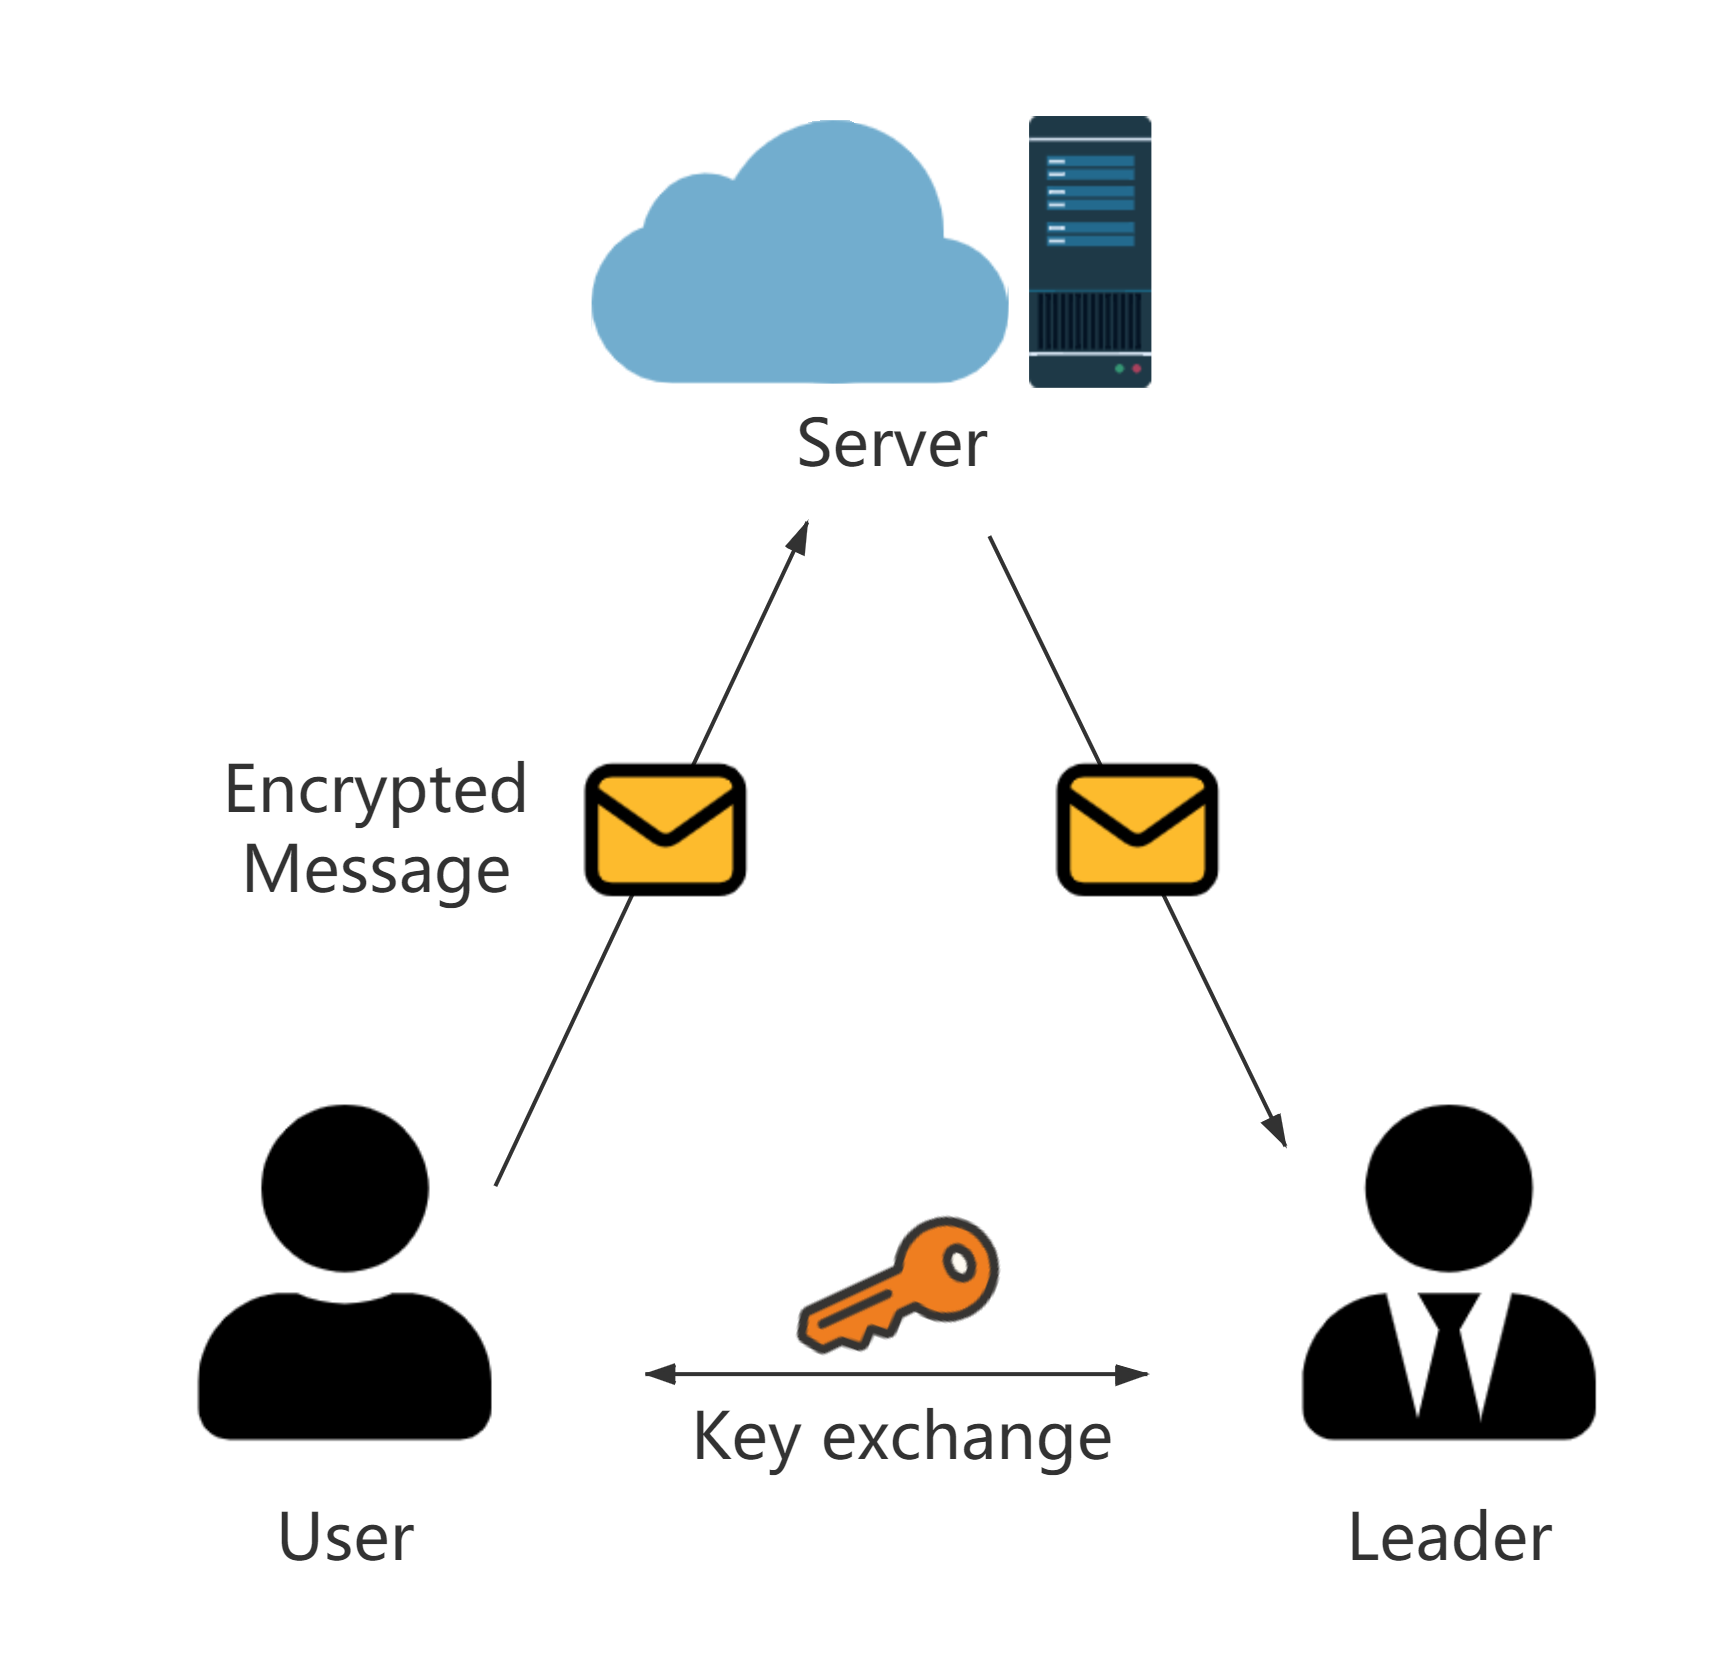
\includegraphics[width=\columnwidth]{img/leader-user.png}
    \caption{The institution can communicate with all users directly while all the leader-user pair share a secret key used for private communication. The server helps to forward encrypted messages from which it can know nothing.}
    \label{leader-user}
\end{figure}

\subsubsection{\textbf{Key exchange}}
When the parties receive $L$, they will know who the leaders are. In order to communicate with the leaders privately, the parties need to run key-exchange protocols to share secret keys. We employ Diffie-Hellman (DH) protocol~\cite{DH} to realize it. 
% Google has experimented with DH in federated learning~\cite{Practical} and there are some techniques to improve the performance, which our framework will also adopt.

In a server-based environment, a server can communicate with any clients while the parties are unfamiliar with each other. Therefore, the key exchange process should be conducted in virtue of the server. In the premise that the server is honest-but-curious, parties can exchange keys in a ``man-in-the-middle'' scheme, where the ``man'' is the honest server. The server delivers information for the parties and leaders. This process is secure because information leaked to the server in key-exchange protocols is useless.

After the key exchange process, each party-leader pair, a party $P_i$ with a leader $L_j$ will share a secret key $K_{ij}$. By means of $K_{ij}$ the party $P_i$ and leader $L_j$ can encrypt their data against the honest-but-curious attacker. The message $m$ can be encrypted as $Enc_{K_{ij}}(m)$. Figure~\ref{leader-user} illustrates the institution-leader-user structure. Normally, the institution and the common users only need to communicate with the leaders.

\subsubsection{\textbf{Secure learning}}
The learning method is based on FedAvg algorithm~\cite{mcmahan2016communicationefficient}. A secure multi-party addition protocol is used to realize privacy-preserving. There are $N_l$ leaders in the system. Without loss of generality, we suppose $N_l = 3$. The flow chart of secure learning process is shown in Figure~\ref{fig-alg} and the process is illustrated as below:

\begin{enumerate}
    \item All the selected parties train the model locally. And a party $P_i$ will get a parameter $G_i$.
    
    \item Each $G_i$ is divided into 3 pieces $G_{i1}$, $G_{i2}$ and $G_{i3}$, where $G_i = G_{i1} + G_{i2} + G_{i3}$. Then $G_{ij}$ is sent to the $j^{th}$ leader $L_j$ respectively.
    
    \item A leader $L_j$ will record a set $B_j$, which consists of the parties that have sent messages to $L_j$. When all the parties' parameters are sent or time is up, the leaders will send $B_j$s to the server and the server will compute the intersection as $B$. Then $B$ is sent back to all leaders. Each leader reserve parameter shares according to $B$ in case that some parties did not send parameter pieces to all leaders successfully. 

    Parties not included in the intersection are then removed. 

    \item Leader $L_j$ then computes the sum of the parameters $A_j = \sum_{i=1}^nG_{ij}$. Afterwards, $A_j$ will be sent to the server.

    \item The server computes: 
    $$W_{global} = \frac{A_1 + A_2 + A_3}{C}  = \frac{\sum_{i=1}^nG_i}{C} $$ 
    and it is the target of FedAvg algorithm. $W_{global}$ is used to update the global model and the server will prepare for the next learning round.
\end{enumerate}

$C$ can be obtained in the same manner: replace $G_i$ with $C_i$ and the server can get $C$ privately. In fact, $C_i$ and $G_i$ are sent to leaders at the same time. Alternatively, $C_i$s can also be directly sent to the server without encrypted since they do not help attackers understanding the parameters. When the system decides to discard a party $P_i$ due to $B$, it also needs to discard $C_i$, which will change the amount of training data $C$. The pseudocode of secure learning is illustrated in Algorithm ~\ref{sec-learning}. Neither the server nor any leader can figure out what exactly a certain party's parameter is based on the information it can receive. 

\begin{figure*}[!ht]
    \centering
    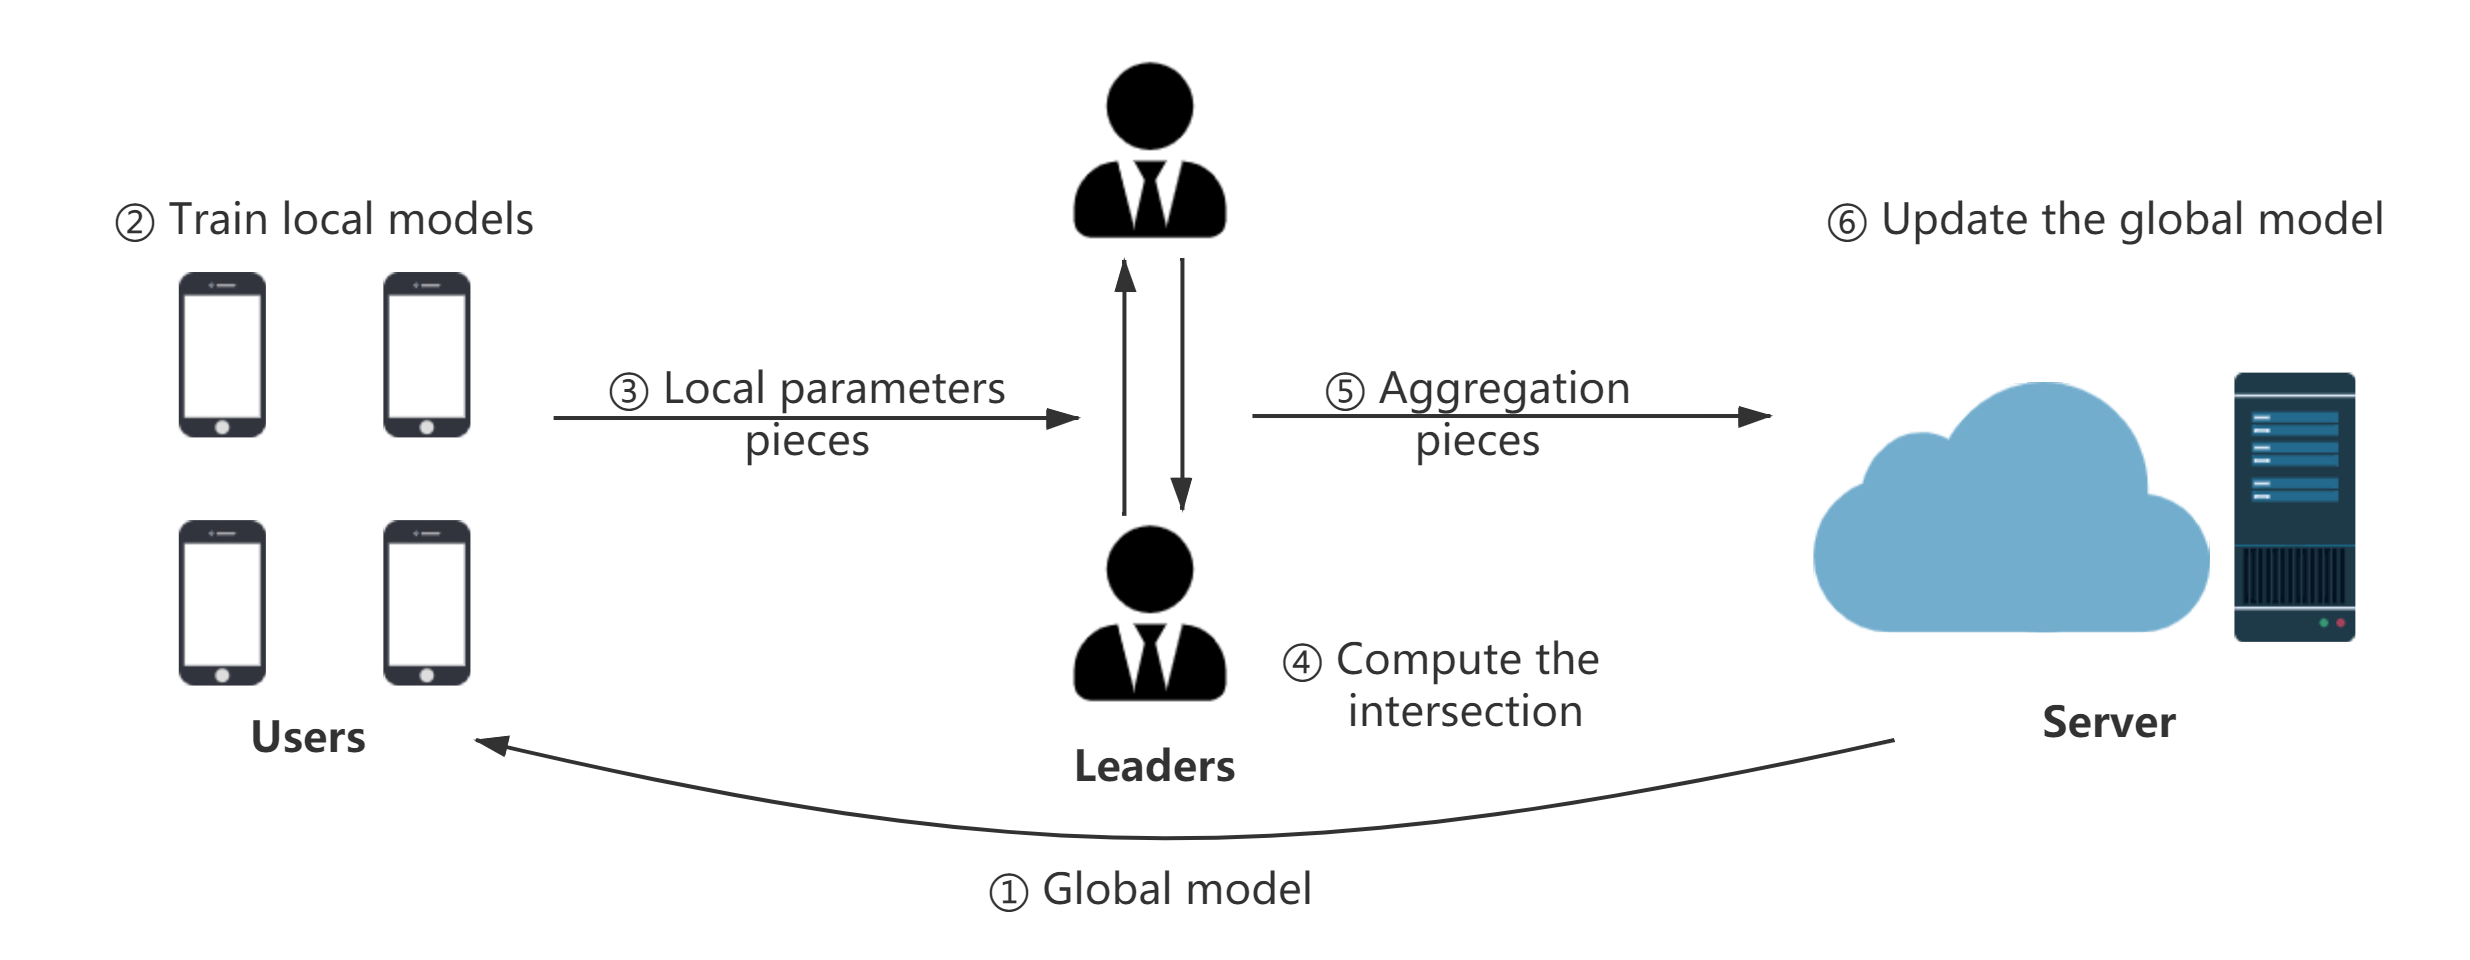
\includegraphics[width=2\columnwidth]{img/alg.png}
    \caption{The flow chart of the secure learning process. It is based on the fact that common users have already constructed secure communication channels with leaders. After step 6, the process will enter the next epoch and restart from step 1.}
    \label{fig-alg}
\end{figure*}

\begin{algorithm}
    \label{sec-learning}
    \caption{Secure Learning Algorithm}
    \begin{algorithmic}[1] 
        \Require $G_i$, $L$, $K_i$ (the set of secret keys for party $P_i$), $E_{max}$ (the maximum epoch for federated learning)
        \Function {split\_parameter}{$G_i$}
            \State $r \gets \Call{random}{0, 0.5}$
            \State $G_{i1} \gets G_i * r$
            \State $r \gets \Call{random}{0, 1-r}$
            \State $G_{i2} \gets G_i * r$
            \State $G_{i3} \gets G_i - G_{i1} - G_{i2}$
            \State \Return{$G_{i1}, G_{i2}, G_{i3}$}
        \EndFunction
        \State
        \Function {party\_send}{$G_i, L, K_i$}
            \State $G_{i1}, G_{i2}, G_{i3} \gets$ \Call{split\_parameter}{$G_i$}
            \For {$j \in$ indexes of $L$}
                \State $E_{ij} \gets \Call{Enc}{K_{ij}, G_{ij}}$
                \If {Sends $E_{ij}$ to $L_j$ not successfully}
                    \State Report ``$L_j$ is crashed'' to $S$
                \EndIf
            \EndFor
        \EndFunction
        \State
        \Function {leader\_send}{$K_j$}
            \State $B_j \gets \emptyset$
            \State Receive $E_{ij}$s from all possible $P_i$ and add $i$ to $B_j$
            \State Send $B_j$ to $S$
            \State Receive $B$ from $S$
            \State Remove $E_{ij}$s whose $i$ is not included in $B$
            \State $G_{ij} \gets \Call{Dec}{K_{ij}, E_{ij}}$ for each $E_{ij}$
            \State $A_j \gets \sum_{i=1}^nG_{ij}$
            \State Sends $A_j$ to $S$
        \EndFunction
        \State
        \Function {server\_aggregation}{e}
            \If{$e \ge E_{max}$}
                \State \Return{$True$}
            \EndIf
            \State Receive $A_j$s from leaders
            \State $W_{global} \gets \frac{A_1 + A_2 + A_3}{C} $
            \State \Call{Update}{$Model_{global}, W_{global}$} 
            \State $//$ Next epoch
            \State Select $n$ parties to participate in the next epoch
            \State Send $W_{global}$ to these $n$ parties
            \State \Return{\Call{server\_aggregation}{e+1}}
        \EndFunction
    \end{algorithmic}
\end{algorithm}


\subsubsection{\textbf{Reorganization}}
The reorganization process provides the robustness for the framework. Normally, the server will notice a leader's crash within a heart-beat cycle. Meanwhile, a party will report to the server if it finds a leader is crashed. After noticing a leader is crashed, the server sends ``stop'' signals to all parties, and randomly select a new party as the new leader. $L$ will be updated and sent to all common parties. Finally, the learning process will be restarted.

\subsection{Among-institutions Model}
Since secure P2P communication is already constructed, the key exchange process is removed in this situation. In addition, consensus algorithms can be executed naturally in such an environment as it is in a decentralized system where parties are equal. Therefore, leaders are elected by voting as the original Raft does. The leader-tenure and reorganization processes also vote for new leaders instead of getting leaders from a server.

